\section{Implementation of the experiments}


In our program, many options are parametrizable. Those can be set using program arguments :
\begin{itemize}
\item The graph to play on (graphviz format supported)
\item The number of colors to play with
\item The number of games to play
\item The number of simulations to be run by Monte-Carlo before selecting a move
\end{itemize}
After some testing, we settled on the following experimental conditions :
\begin{itemize}
\item A number of simulations of 1000. This seemed to be a good compromise between speed and AI accuracy.
\item A number of games played of 1000. It seemed again to be a good compromise between computation time and statistical confidence. However, we could not play as many games on the 5x5 grids with a high number of colors (typically 4 or 5). We then tuned down the games to 100 for those cases. 
\end{itemize}

Here are the results :\\

\subsection{Chains}

\subsubsection{Odd number of vertices}

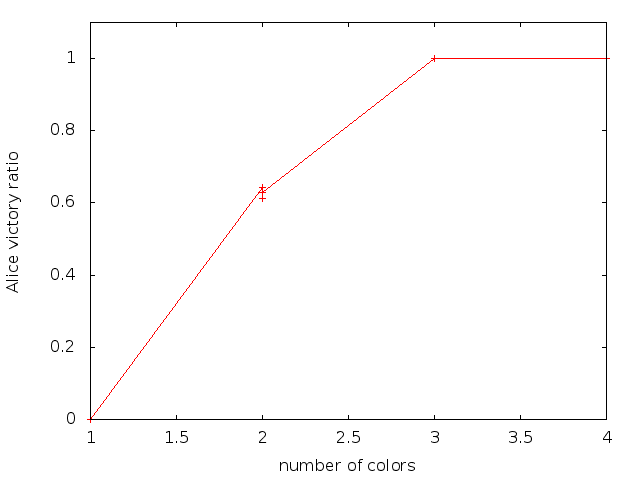
\includegraphics[width=11cm]{resultats/chaineimpaire.png}

\subsubsection{Even number of vertices}

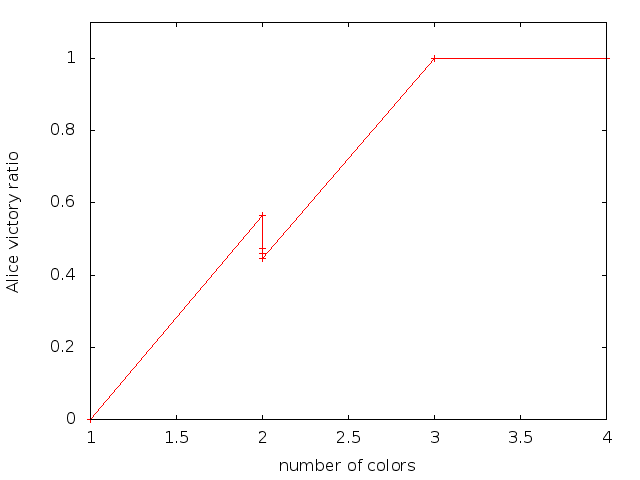
\includegraphics[width=11cm]{resultats/chainepaire.png}

The chains are 2-coloriable graphs. However, we can see on those curves that 2 colors are not enough for Alice to win every time. Due to the simplicity of the graph, 3 colors seem to be sufficient regardless of the number of vertices in the graph.

\subsection{Cycles}

\subsubsection{Odd number of vertices}

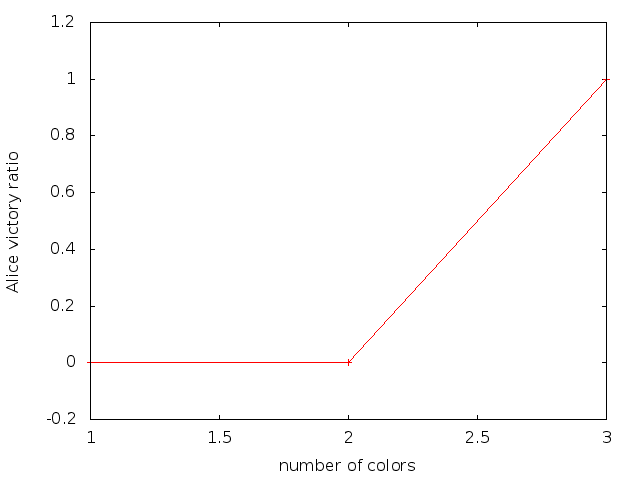
\includegraphics[width=11cm]{resultats/cycleimpair.png}

An odd cycle is not 2-coloriable, but suprisingly Alice seems to win every time with only 3 colors, which is the minimal amount to achieve a proper coloring. This means that Bob cannot win on an odd cycle.

\subsubsection{Even number of vertices}

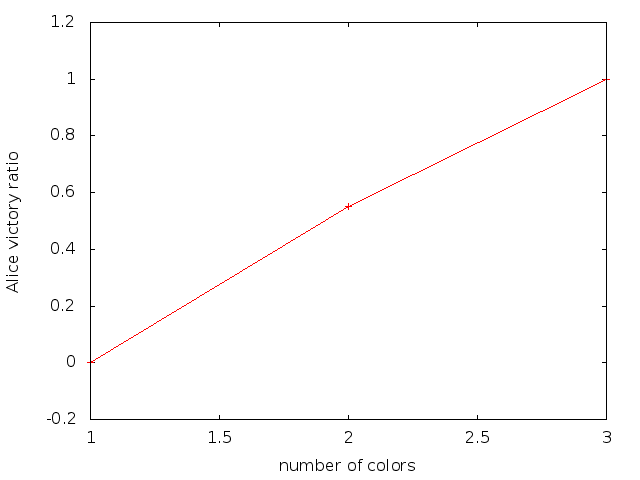
\includegraphics[width=11cm]{resultats/cyclepair.png}

An even cycle demands at least 2 colors to be properly colored. But this time, Alice only achieves a 0.5 ratio with 2 colors. She needs 3 colors to be able to beat Bob on every game.

\subsection{Grids}

\subsubsection{2x5}

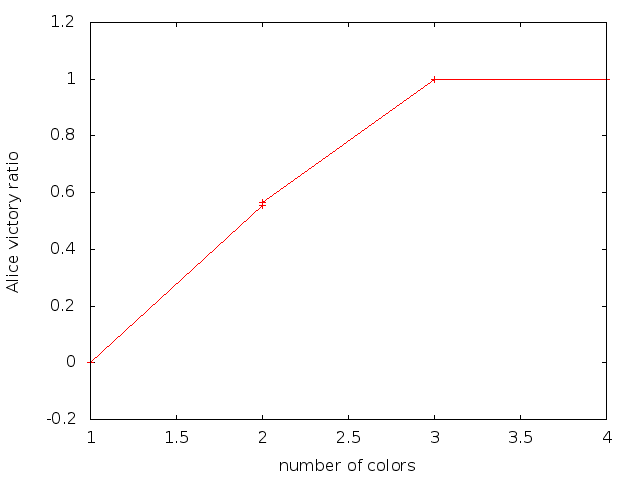
\includegraphics[width=11cm]{resultats/grille25.png}

This little grid is quite similar to an odd cycle : 2-coloriable and Alice wins with 3 colors. This is propably because of the little size of the grid.

\subsubsection{5x5}

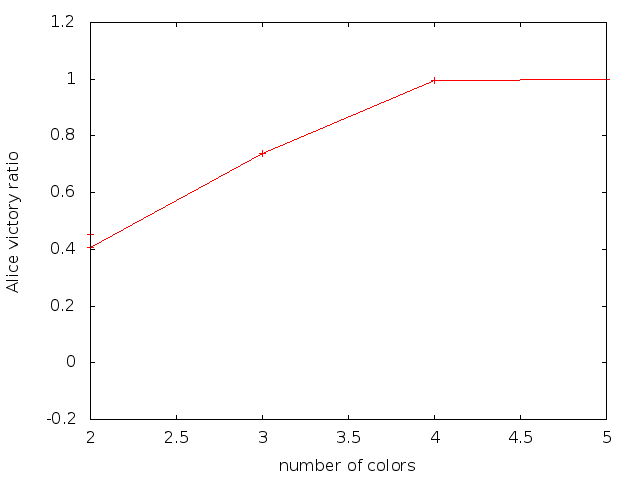
\includegraphics[width=11cm]{resultats/grille55.png}

This grid is bigger than the previous one. This can be seen on the results : while still being 2-coloriable, our Alice needs at least 5 colors to be able to win every time. Moreover her ratio with 3 colors is only about 0.7 and with 4 colors it is very close but still under a perfect 1 ratio. From this we can conclude that the game chromatic number of this grid is certainly around 4 or 5.

\subsubsection{5x5 toroidal}

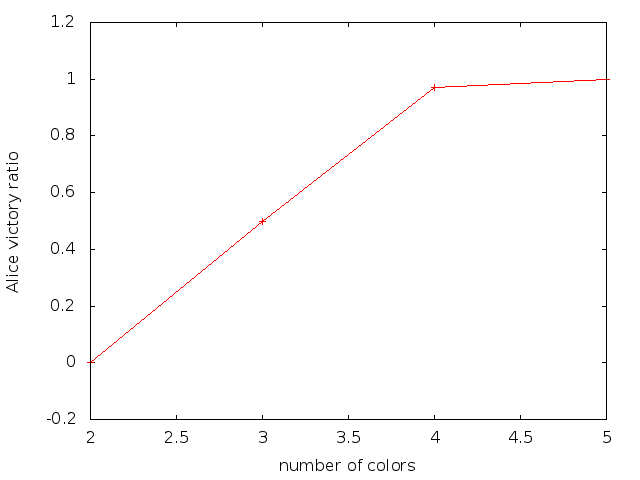
\includegraphics[width=11cm]{resultats/grilletor55.png}

The toroidal nature of this grid implies that its chromatic number is 3. The game chromatic number of toroidal grids has been proved to be 5 in \cite{Raspaud20091183}. This result is confirmed by our data. Indeed, 5 is the least number of colors for wich Alice achieves a 1 ratio.

\subsection{Binary Tree}

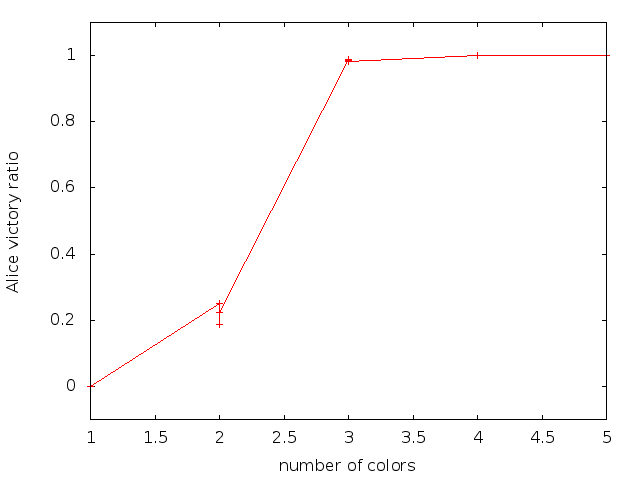
\includegraphics[width=11cm]{resultats/bintree3h.png}

\subsection{Non-Planar Graphs}

\subsubsection{Petersen Graph}

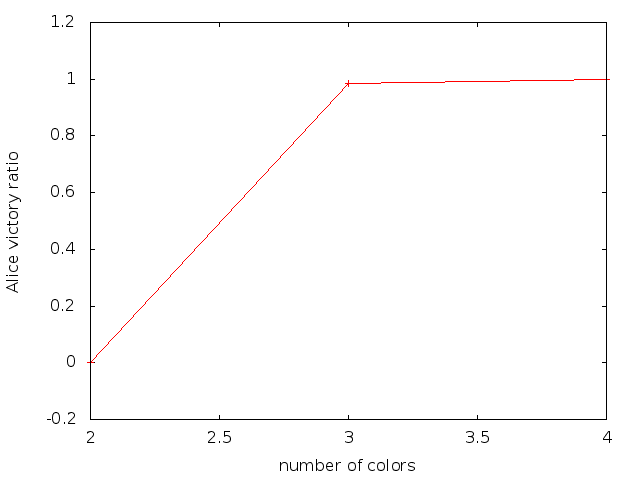
\includegraphics[width=11cm]{resultats/petersen.png}

Alice needed 4 colors for the perfect ratio, but 3 is not far behind. However, 4 is still far under the bounds of the original article.

\subsubsection{Icosaedron Graph}

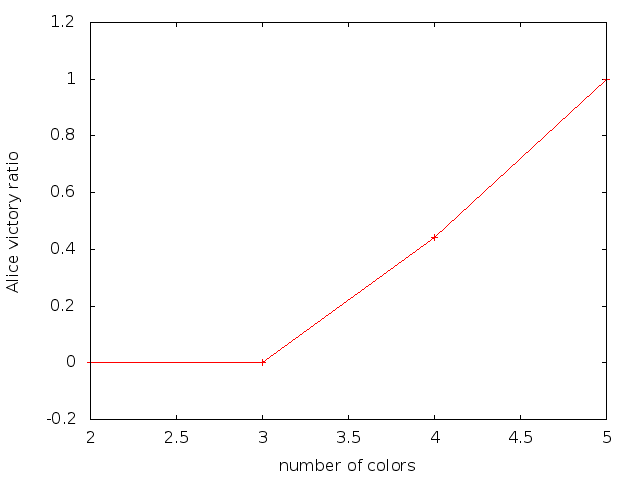
\includegraphics[width=11cm]{resultats/icosaedre.png}

This graph seemed to be the most difficult for Alice. Her ratio with 4 colors is only 0.4. She wins every time with 5, but the bounds of the article are greater. Maybe the real game chromatic number is between 5 and the article's bounds.